%geo 1
Finndu flatarmál skyggða svæðisins.
\begin{center}
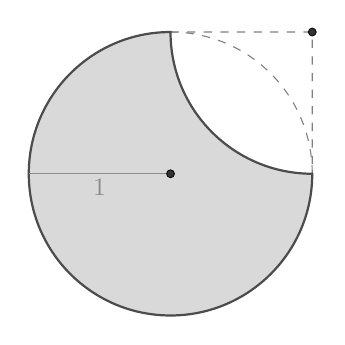
\begin{tikzpicture}[scale=1.8,
    dot/.style={circle, fill=black!80, draw=black, line width=0.3pt, inner sep=1pt},
    lbl/.style={font=\small, inner sep=2pt}]
  % --- data: circle of radius 1 centred at O; quarter circle of radius 1 centred at K=(1,1) ---
  \coordinate (O) at (0,0);
  \coordinate (K) at (1,1);

  % --- shaded region: circle minus the quarter disc centred at K ---
  \fill[black!15]
    (0,1) arc[start angle=90, end angle=360, radius=1]
          arc[start angle=270, end angle=180, radius=1] -- cycle;

  % --- drawing ---
  \draw[gray, dashed] (1,0) arc[start angle=0, end angle=90, radius=1]; % removed part of circle
  \draw[gray, dashed] (0,1) -- (K) -- (1,0);                           % corner square
  \draw[black!70, thick]
    (0,1) arc[start angle=90, end angle=360, radius=1]
          arc[start angle=270, end angle=180, radius=1] -- cycle;
  \draw[black!45] (O) -- node[lbl, below] {$1$} (-1,0);

  \node[dot] at (O) {};
  \node[dot] at (K) {};
\end{tikzpicture}
\end{center}
